\chapter{Introduction}
\label{chap:intro}

Over the past few years, conversational agents have grown in importance, conquering the world of technology by finally being available even in the smallest of devices that everyone has nowadays, smartphones.
Conversational agents have been widely used for years in a variety of applications even before smartphones came by, like phone call routing and other simple, limited domain applications.
But in the smartphones age, all of today's smartphones ship with a virtual voice assistant as big tech companies such as Google, Microsoft and Apple compete in providing the most functionality through such assistants, enabling their users to control their phones hands-free.
However, most of these advancements are proprietary software and the open source community is yet to catch up.

This work describes Halef\cite{modernconvagents}, an open source, industry standards compliant spoken dialog system\cite{opensrcsds}\cite{archopensrcsds}, which aims at bridging that gap between proprietary software and it's open source counterpart.
Halef works in a unique distributed architecture, splitting it into three main components, with the ability to split those three main components even further giving a high degree of flexibility and easily allowing multiple different architectures to suit each use case.
In addition to all that, all protocols that Halef runs on; SIP and MRCP/RTP, are industry standards compliant, making it suitable and trusted for use in industry as well as research.
The Halef application development language, \ac{vxml}, is also widely recognized in the community and many proprietary softwares out there already use it as well to define their applications.
So, with all that in mind, we will jump into the nitty gritty details of Halef in the next few sections, describing how it works as well as how to tweak it for use in different areas of application with a variety of distributed architectures.

\section{Background - General Halef Architecture}
\begin{figure}[h]
  \centering
  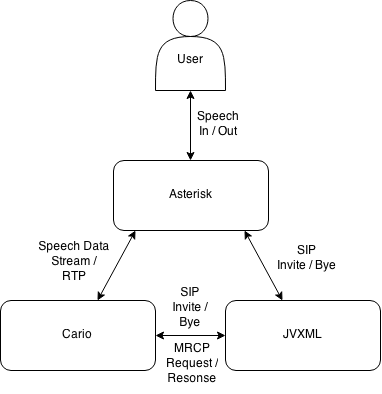
\includegraphics[width=11cm]{resources/images/Halef-General.png}
  \caption{Halef's General Architecture}
  \label{fig:halefgeneral}
\end{figure}

As mentioned earlier, Halef is composed of three main servers; Cairo, JVXML and Asterisk.
Those three servers interact in different ways to provide the final functionality of Halef.
In this section, a brief description of the role of each server will be given, in addition to how they all interact to provide Halef's functionality.

\subsection{The Asterisk Server}
Asterisk is a free, open source framework that provides the functionality of a telephony server servicing multiple types of connections like SIP, IP PBX and \ac{pstn}.
The Asterisk project is widely used and recognized by industry, governments and the open source community.
It has a large user base, providing a lot of support over the forums and the project itself is also documented very well.
You can read more about the Asterisk project on its website\footnote{http://www.asterisk.org/} and the book "Asterisk: A Definitive Guide"\cite{asterisk}.
In the case of Halef, regular phone calls over \ac{pstn} and VoIP calls over SIP are supported.
Users can call in to Halef using their telephones or cellphones on the US number assigned to it, or they can call in free using a SIP softphone utilising the provided VoIP service.
Either way, the Asterisk server serves as the entry point of a user call into Halef.
When a user calls in over PSTN or SIP, the Asterisk telephony server picks up the call, welcomes the user then asks for an extension to route the user to.
Each extension points to a different Halef instance running its own application, providing a robust way of running different Halef instances but connecting them all to the same telephony service that is set up on a single server.
This reduces the work needed down to only integrating the needed JVXML and Cairo servers with the already running telephony server.

\subsection{The Cairo Server}
The Cairo server is the core of Halef, being responsible for both speech recognition and synthesis.
When the call is set up, the Cairo server is connected to the JVXML server over MRCP channels to receive recogntion and synthesis requests, and to the Asterisk Server over RTP to stream audio back and forth to and from the user.
When the Cairo server receives an MRCP recognition request, it chooses the suitable recognizer type specified in the MRCP message through the recognition interface then segments the open RTP stream to detect the speech utterance to recognize, then returns the recognition result to JVXML.
On the other hand, when it receives a synthesis request, it synthesizes the string specified in the MRCP message then streams the synthesized speech to the user through Asterisk, over RTP.
The Cairo Server will be described in detail in Chapter \ref{chap:cairo}.

\subsection{The JVXML Server}
JVXML is an open-source voice browser for \ac{vxml} written in Java.
It works as a \ac{vxml} interpreter, parsing and executing the \ac{vxml} applications written to Halef and specified in the JVXML Server's configuration file.
The JVXML Server connects to Asterisk through SIP and to Cairo through both SIP and MRCP.
Once a user call is received, Asterisk connects to the JVXML Server through SIP, which then forwards the SIP messages to the Cairo server to set up its MRCP and RTP channels.
The JVXML server then goes on to parse and execute the specified application, sending recognition and syntesis requests to Cairo over MRCP when the application requests either action.

\subsection{Interaction between the Servers}
The three servers are interconnected over different channels that set up then provide Halef's functionality throughout the user's call.
The first connection is between the Asterisk and the JVXML servers.
Those two servers are connect via SIP, which is used to signal the start and end of a call, as well as provide the information needed to set up the RTP session.
The SIP messages sent from the Asterisk server to the JVXML one are then forwarded by JVXML to the Cairo server.
The Cairo server then uses the information in the messages to allocate and free resources as requested.
The second connection is between the Cairo and Asterisk servers.
This connection is over RTP, which is used to send the user's speech stream to Cairo and return the synthesized text prompt to Asterisk so it can play it to the user.
The third essential conncection is between Cairo and JVXML.
This connection is over MRCP which enables JVXML to send Cairo speech specific requests such as \textit{RECOGNIZE}, \textit{RECORD} and \textit{SYNTHESIZE}.
Cairo then returns the results of those operations, such as the recognized text for a \textit{RECOGNIZE} request, to JVXML over MRCP as well. 

\section{Objectives} \label{sec:s1}
The main goal of this work is to describe Halef in as much detail as possible, from the conceptual and architectural level, to the classes distribution and actual code level.
With three independent servers forming the backbone of Halef, each will be described in detail as to how it runs, its own architecture and finally, how it works to serve the requests it receives to contribute to the work of the whole system.
Several practices and areas for change and improvement will be pointed out throughout the whole book and finally summarized in the final chapters.
Some applications that have been integrated and tested with Halef will also be included to demonstrate how Halef can serve different applications as well as how to overcome some difficulties with needed features that are not part of the system yet.

\section{Structure}
This book starts the walk through Halef by describing the first server, the Cairo server, in chapter \ref{chap:cairo}.
This chapter will go into Cairo's architecture and how to start its different components.
It then describes the life cycle of the five main requests this server has to handle, the SIP invite, SIP bye, MRCP recognize, MRCP record and MRCP synthesize requests.
\par
The next chapter, \ref{chap:jvxml}, describes the JVXML server, starting from parsing the application file to communicating with the Cairo server to satisfy the recognition and synthesis requests.
\par
Finally, some applications that have been already integrated into Halef will be described, in addition to the suggested future work on the system, before concluding the book.
